\documentclass[11pt,fleqn, oneside,openany]{book} % Default font size and left-justified equations

% use this list: https://www.educative.io/blog/google-coding-interview

%%%%%%%%%%%%%%%%%%%%%%%%%%%%%%%%%%%%%%%%%%%%
%               Structure
%%%%%%%%%%%%%%%%%%%%%%%%%%%%%%%%%%%%%%%%%%%%
%%%%%%%%%%%%%%%%%%%%%%%%%%%%%%%%%%%%%%%%%
% The Legrand Orange Book
% Structural Definitions File
% Version 2.0 (9/2/15)
%
% Original author:
% Mathias Legrand (legrand.mathias@gmail.com) with modifications by:
% Vel (vel@latextemplates.com)
% 
% This file has been downloaded from:
% http://www.LaTeXTemplates.com
%
% License:
% CC BY-NC-SA 3.0 (http://creativecommons.org/licenses/by-nc-sa/3.0/)
%
%%%%%%%%%%%%%%%%%%%%%%%%%%%%%%%%%%%%%%%%%

%----------------------------------------------------------------------------------------
%	VARIOUS REQUIRED PACKAGES AND CONFIGURATIONS
%----------------------------------------------------------------------------------------

\usepackage[top=3cm,bottom=3cm,left=3cm,right=3cm,headsep=10pt,a4paper]{geometry} % Page margins

\usepackage{graphicx} % Required for including pictures
\graphicspath{{images/}} % Specifies the directory where pictures are stored

\usepackage{lipsum} % Inserts dummy text

\usepackage{tikz} % Required for drawing custom shapes

\usepackage[english]{babel} % English language/hyphenation

\usepackage{enumitem} % Customize lists
\setlist{nolistsep} % Reduce spacing between bullet points and numbered lists

\usepackage{booktabs} % Required for nicer horizontal rules in tables

\usepackage{xcolor} % Required for specifying colors by name
\definecolor{ocre}{RGB}{243,102,25} % Define the orange color used for highlighting throughout the book

%----------------------------------------------------------------------------------------
%	FONTS
%----------------------------------------------------------------------------------------

\usepackage{avant} % Use the Avantgarde font for headings
%\usepackage{times} % Use the Times font for headings
\usepackage{mathptmx} % Use the Adobe Times Roman as the default text font together with math symbols from the Sym­bol, Chancery and Com­puter Modern fonts

\usepackage{microtype} % Slightly tweak font spacing for aesthetics
\usepackage[utf8]{inputenc} % Required for including letters with accents
\usepackage[T1]{fontenc} % Use 8-bit encoding that has 256 glyphs

%----------------------------------------------------------------------------------------
%	BIBLIOGRAPHY AND INDEX
%----------------------------------------------------------------------------------------

\usepackage[citestyle=numeric,sorting=nyt,sortcites=true,autopunct=true,babel=hyphen,hyperref=true,abbreviate=false,backref=true,backend=biber]{biblatex}
\addbibresource{sources/bibliography.bib}
\defbibheading{bibempty}{}

\usepackage{calc} % For simpler calculation - used for spacing the index letter headings correctly
\usepackage{makeidx} % Required to make an index
\makeindex % Tells LaTeX to create the files required for indexing

%----------------------------------------------------------------------------------------
%	MAIN TABLE OF CONTENTS
%----------------------------------------------------------------------------------------

\usepackage{titletoc} % Required for manipulating the table of contents

\contentsmargin{0cm} % Removes the default margin

% Part text styling
\titlecontents{part}[0cm]
{\addvspace{20pt}\centering\large\bfseries}
{}
{}
{}

% Chapter text styling
\titlecontents{chapter}[1.25cm] % Indentation
{\addvspace{12pt}\large\sffamily\bfseries} % Spacing and font options for chapters
{\color{ocre!60}\contentslabel[\Large\thecontentslabel]{1.25cm}\color{ocre}} % Chapter number
{\color{ocre}}  
{\color{ocre!60}\normalsize\;\titlerule*[.5pc]{.}\;\thecontentspage} % Page number

% Section text styling
\titlecontents{section}[1.25cm] % Indentation
{\addvspace{3pt}\sffamily\bfseries} % Spacing and font options for sections
{\contentslabel[\thecontentslabel]{1.25cm}} % Section number
{}
{\hfill\color{black}\thecontentspage} % Page number
[]

% Subsection text styling
\titlecontents{subsection}[1.25cm] % Indentation
{\addvspace{1pt}\sffamily\small} % Spacing and font options for subsections
{\contentslabel[\thecontentslabel]{1.25cm}} % Subsection number
{}
{\ \titlerule*[.5pc]{.}\;\thecontentspage} % Page number
[]

% List of figures
\titlecontents{figure}[0em]
{\addvspace{-5pt}\sffamily}
{\thecontentslabel\hspace*{1em}}
{}
{\ \titlerule*[.5pc]{.}\;\thecontentspage}
[]

% List of tables
\titlecontents{table}[0em]
{\addvspace{-5pt}\sffamily}
{\thecontentslabel\hspace*{1em}}
{}
{\ \titlerule*[.5pc]{.}\;\thecontentspage}
[]

%----------------------------------------------------------------------------------------
%	MINI TABLE OF CONTENTS IN PART HEADS
%----------------------------------------------------------------------------------------

% Chapter text styling
\titlecontents{lchapter}[0em] % Indenting
{\addvspace{15pt}\large\sffamily\bfseries} % Spacing and font options for chapters
{\color{ocre}\contentslabel[\Large\thecontentslabel]{1.25cm}\color{ocre}} % Chapter number
{}  
{\color{ocre}\normalsize\sffamily\bfseries\;\titlerule*[.5pc]{.}\;\thecontentspage} % Page number

% Section text styling
\titlecontents{lsection}[0em] % Indenting
{\sffamily\small} % Spacing and font options for sections
{\contentslabel[\thecontentslabel]{1.25cm}} % Section number
{}
{}

% Subsection text styling
\titlecontents{lsubsection}[.5em] % Indentation
{\normalfont\footnotesize\sffamily} % Font settings
{}
{}
{}

%----------------------------------------------------------------------------------------
%	PAGE HEADERS
%----------------------------------------------------------------------------------------

\usepackage{fancyhdr} % Required for header and footer configuration

\pagestyle{fancy}
\renewcommand{\chaptermark}[1]{\markboth{\sffamily\normalsize\bfseries\chaptername\ \thechapter.\ #1}{}} % Chapter text font settings
\renewcommand{\sectionmark}[1]{\markright{\sffamily\normalsize\thesection\hspace{5pt}#1}{}} % Section text font settings
\fancyhf{} \fancyhead[LE,RO]{\sffamily\normalsize\thepage} % Font setting for the page number in the header
\fancyhead[LO]{\rightmark} % Print the nearest section name on the left side of odd pages
\fancyhead[RE]{\leftmark} % Print the current chapter name on the right side of even pages
\renewcommand{\headrulewidth}{0.5pt} % Width of the rule under the header
\addtolength{\headheight}{2.5pt} % Increase the spacing around the header slightly
\renewcommand{\footrulewidth}{0pt} % Removes the rule in the footer
\fancypagestyle{plain}{\fancyhead{}\renewcommand{\headrulewidth}{0pt}} % Style for when a plain pagestyle is specified

% Removes the header from odd empty pages at the end of chapters
\makeatletter
\renewcommand{\cleardoublepage}{
\clearpage\ifodd\c@page\else
\hbox{}
\vspace*{\fill}
\thispagestyle{empty}
\newpage
\fi}

%----------------------------------------------------------------------------------------
%	THEOREM STYLES
%----------------------------------------------------------------------------------------


\usepackage{amsmath,amsfonts,amssymb,amsthm,mathtools} % For math equations, theorems, symbols, etc
\DeclarePairedDelimiter\ceil{\lceil}{\rceil}
\DeclarePairedDelimiter\floor{\lfloor}{\rfloor}

\newcommand{\intoo}[2]{\mathopen{]}#1\,;#2\mathclose{[}}
\newcommand{\ud}{\mathop{\mathrm{{}d}}\mathopen{}}
\newcommand{\intff}[2]{\mathopen{[}#1\,;#2\mathclose{]}}
\newtheorem{notation}{Notation}[chapter]

% Boxed/framed environments
\newtheoremstyle{ocrenumbox}% % Theorem style name
{0pt}% Space above
{0pt}% Space below
{\normalfont}% % Body font
{}% Indent amount
{\small\bf\sffamily\color{ocre}}% % Theorem head font
{\;}% Punctuation after theorem head
{0.25em}% Space after theorem head
{\small\sffamily\color{ocre}\thmname{#1}\nobreakspace\thmnumber{\@ifnotempty{#1}{}\@upn{#2}}% Theorem text (e.g. Theorem 2.1)
\thmnote{\nobreakspace\the\thm@notefont\sffamily\bfseries\color{black}---\nobreakspace#3.}} % Optional theorem note
\renewcommand{\qedsymbol}{$\blacksquare$}% Optional qed square

\newtheoremstyle{blacknumex}% Theorem style name
{5pt}% Space above
{5pt}% Space below
{\normalfont}% Body font
{} % Indent amount
{\small\bf\sffamily}% Theorem head font
{\;}% Punctuation after theorem head
{0.25em}% Space after theorem head
{\small\sffamily{\tiny\ensuremath{\blacksquare}}\nobreakspace\thmname{#1}\nobreakspace\thmnumber{\@ifnotempty{#1}{}\@upn{#2}}% Theorem text (e.g. Theorem 2.1)
\thmnote{\nobreakspace\the\thm@notefont\sffamily\bfseries---\nobreakspace#3.}}% Optional theorem note

\newtheoremstyle{blacknumbox} % Theorem style name
{0pt}% Space above
{0pt}% Space below
{\normalfont}% Body font
{}% Indent amount
{\small\bf\sffamily}% Theorem head font
{\;}% Punctuation after theorem head
{0.25em}% Space after theorem head
{\small\sffamily\thmname{#1}\nobreakspace\thmnumber{\@ifnotempty{#1}{}\@upn{#2}}% Theorem text (e.g. Theorem 2.1)
\thmnote{\nobreakspace\the\thm@notefont\sffamily\bfseries---\nobreakspace#3.}}% Optional theorem note

% Non-boxed/non-framed environments
\newtheoremstyle{ocrenum}% % Theorem style name
{5pt}% Space above
{5pt}% Space below
{\normalfont}% % Body font
{}% Indent amount
{\small\bf\sffamily\color{ocre}}% % Theorem head font
{\;}% Punctuation after theorem head
{0.25em}% Space after theorem head
{\small\sffamily\color{ocre}\thmname{#1}\nobreakspace\thmnumber{\@ifnotempty{#1}{}\@upn{#2}}% Theorem text (e.g. Theorem 2.1)
\thmnote{\nobreakspace\the\thm@notefont\sffamily\bfseries\color{black}---\nobreakspace#3.}} % Optional theorem note
\renewcommand{\qedsymbol}{$\blacksquare$}% Optional qed square
\makeatother

% Defines the theorem text style for each type of theorem to one of the three styles above
\newcounter{dummy} 
\numberwithin{dummy}{section}
\theoremstyle{ocrenumbox}
\newtheorem{theoremeT}[dummy]{Theorem}

\newtheorem{problem}{Exercise}[chapter]
\newtheorem{exerciseT}{Problem}
\theoremstyle{blacknumex}
\newtheorem{solution}{Solution}[chapter]
\newtheorem{solutionT}{solution}[chapter]
\theoremstyle{blacknumex}
\newtheorem{exampleT}{Example}[chapter]
\theoremstyle{blacknumbox}
\newtheorem{vocabulary}{Vocabulary}[chapter]
\newtheorem{definitionT}{Definition}[section]
\newtheorem{corollaryT}[dummy]{Corollary}
\theoremstyle{ocrenum}
\newtheorem{proposition}[dummy]{Proposition}

%----------------------------------------------------------------------------------------
%	DEFINITION OF COLORED BOXES
%----------------------------------------------------------------------------------------

\RequirePackage[framemethod=default]{mdframed} % Required for creating the theorem, definition, exercise and corollary boxes

% Theorem box
\newmdenv[skipabove=7pt,
skipbelow=7pt,
backgroundcolor=black!5,
linecolor=ocre,
innerleftmargin=5pt,
innerrightmargin=5pt,
innertopmargin=5pt,
leftmargin=0cm,
rightmargin=0cm,
innerbottommargin=5pt]{tBox}

% Exercise box	  
\newmdenv[skipabove=7pt,
skipbelow=7pt,
rightline=false,
leftline=true,
topline=false,
bottomline=false,
backgroundcolor=ocre!10,
linecolor=ocre,
innerleftmargin=5pt,
innerrightmargin=5pt,
innertopmargin=5pt,
innerbottommargin=5pt,
leftmargin=0cm,
rightmargin=0cm,
linewidth=4pt]{eBox}	

% Definition box
\newmdenv[skipabove=7pt,
skipbelow=7pt,
rightline=false,
leftline=true,
topline=false,
bottomline=false,
linecolor=ocre,
innerleftmargin=5pt,
innerrightmargin=5pt,
innertopmargin=0pt,
leftmargin=0cm,
rightmargin=0cm,
linewidth=4pt,
innerbottommargin=0pt]{dBox}	

% Corollary box
\newmdenv[skipabove=7pt,
skipbelow=7pt,
rightline=false,
leftline=true,
topline=false,
bottomline=false,
linecolor=gray,
backgroundcolor=black!5,
innerleftmargin=5pt,
innerrightmargin=5pt,
innertopmargin=5pt,
leftmargin=0cm,
rightmargin=0cm,
linewidth=4pt,
innerbottommargin=5pt]{cBox}

% Creates an environment for each type of theorem and assigns it a theorem text style from the "Theorem Styles" section above and a colored box from above
\newenvironment{theorem}{\begin{tBox}\begin{theoremeT}}{\end{theoremeT}\end{tBox}}
\newenvironment{exercise}{\begin{eBox}\begin{exerciseT}}{\hfill{\color{ocre}\tiny\ensuremath{\blacksquare}}\end{exerciseT}\end{eBox}}				  
\newenvironment{definition}{\begin{dBox}\begin{definitionT}}{\end{definitionT}\end{dBox}}	
\newenvironment{example}{\begin{exampleT}}{\hfill{\tiny\ensuremath{\blacksquare}}\end{exampleT}}		
\newenvironment{corollary}{\begin{cBox}\begin{corollaryT}}{\end{corollaryT}\end{cBox}}	

%----------------------------------------------------------------------------------------
%	REMARK ENVIRONMENT
%----------------------------------------------------------------------------------------

\newenvironment{remark}{\par\vspace{10pt}\small % Vertical white space above the remark and smaller font size
\begin{list}{}{
\leftmargin=35pt % Indentation on the left
\rightmargin=25pt}\item\ignorespaces % Indentation on the right
\makebox[-2.5pt]{\begin{tikzpicture}[overlay]
\node[draw=ocre!60,line width=1pt,circle,fill=ocre!25,font=\sffamily\bfseries,inner sep=2pt,outer sep=0pt] at (-15pt,0pt){\textcolor{ocre}{R}};\end{tikzpicture}} % Orange R in a circle
\advance\baselineskip -1pt}{\end{list}\vskip5pt} % Tighter line spacing and white space after remark

%----------------------------------------------------------------------------------------
%	SECTION NUMBERING IN THE MARGIN
%----------------------------------------------------------------------------------------

\makeatletter
\renewcommand{\@seccntformat}[1]{\llap{\textcolor{ocre}{\csname the#1\endcsname}\hspace{1em}}}                    
\renewcommand{\section}{\@startsection{section}{1}{\z@}
{-4ex \@plus -1ex \@minus -.4ex}
{1ex \@plus.2ex }
{\normalfont\large\sffamily\bfseries}}
\renewcommand{\subsection}{\@startsection {subsection}{2}{\z@}
{-3ex \@plus -0.1ex \@minus -.4ex}
{0.5ex \@plus.2ex }
{\normalfont\sffamily\bfseries}}
\renewcommand{\subsubsection}{\@startsection {subsubsection}{3}{\z@}
{-2ex \@plus -0.1ex \@minus -.2ex}
{.2ex \@plus.2ex }
{\normalfont\small\sffamily\bfseries}}                        
\renewcommand\paragraph{\@startsection{paragraph}{4}{\z@}
{-2ex \@plus-.2ex \@minus .2ex}
{.1ex}
{\normalfont\small\sffamily\bfseries}}

%----------------------------------------------------------------------------------------
%	PART HEADINGS
%----------------------------------------------------------------------------------------

% numbered part in the table of contents
\newcommand{\@mypartnumtocformat}[2]{%
\setlength\fboxsep{0pt}%
\noindent\colorbox{ocre!20}{\strut\parbox[c][.7cm]{\ecart}{\color{ocre!70}\Large\sffamily\bfseries\centering#1}}\hskip\esp\colorbox{ocre!40}{\strut\parbox[c][.7cm]{\linewidth-\ecart-\esp}{\Large\sffamily\centering#2}}}%
%%%%%%%%%%%%%%%%%%%%%%%%%%%%%%%%%%
% unnumbered part in the table of contents
\newcommand{\@myparttocformat}[1]{%
\setlength\fboxsep{0pt}%
\noindent\colorbox{ocre!40}{\strut\parbox[c][.7cm]{\linewidth}{\Large\sffamily\centering#1}}}%
%%%%%%%%%%%%%%%%%%%%%%%%%%%%%%%%%%
\newlength\esp
\setlength\esp{4pt}
\newlength\ecart
\setlength\ecart{1.2cm-\esp}
\newcommand{\thepartimage}{}%
\newcommand{\partimage}[1]{\renewcommand{\thepartimage}{#1}}%
\def\@part[#1]#2{%
\ifnum \c@secnumdepth >-2\relax%
\refstepcounter{part}%
\addcontentsline{toc}{part}{\texorpdfstring{\protect\@mypartnumtocformat{\thepart}{#1}}{\partname~\thepart\ ---\ #1}}
\else%
\addcontentsline{toc}{part}{\texorpdfstring{\protect\@myparttocformat{#1}}{#1}}%
\fi%
\startcontents%
\markboth{}{}%
{\thispagestyle{empty}%
\begin{tikzpicture}[remember picture,overlay]%
\node at (current page.north west){\begin{tikzpicture}[remember picture,overlay]%	
\fill[ocre!20](0cm,0cm) rectangle (\paperwidth,-\paperheight);
\node[anchor=north] at (4cm,-3.25cm){\color{ocre!40}\fontsize{220}{100}\sffamily\bfseries\@Roman\c@part}; 
\node[anchor=south east] at (\paperwidth-1cm,-\paperheight+1cm){\parbox[t][][t]{8.5cm}{
\printcontents{l}{0}{\setcounter{tocdepth}{1}}%
}};
\node[anchor=north east] at (\paperwidth-1.5cm,-3.25cm){\parbox[t][][t]{15cm}{\strut\raggedleft\color{white}\fontsize{30}{30}\sffamily\bfseries#2}};
\end{tikzpicture}};
\end{tikzpicture}}%
\@endpart}
\def\@spart#1{%
\startcontents%
\phantomsection
{\thispagestyle{empty}%
\begin{tikzpicture}[remember picture,overlay]%
\node at (current page.north west){\begin{tikzpicture}[remember picture,overlay]%	
\fill[ocre!20](0cm,0cm) rectangle (\paperwidth,-\paperheight);
\node[anchor=north east] at (\paperwidth-1.5cm,-3.25cm){\parbox[t][][t]{15cm}{\strut\raggedleft\color{white}\fontsize{30}{30}\sffamily\bfseries#1}};
\end{tikzpicture}};
\end{tikzpicture}}
\addcontentsline{toc}{part}{\texorpdfstring{%
\setlength\fboxsep{0pt}%
\noindent\protect\colorbox{ocre!40}{\strut\protect\parbox[c][.7cm]{\linewidth}{\Large\sffamily\protect\centering #1\quad\mbox{}}}}{#1}}%
\@endpart}
\def\@endpart{\vfil\newpage
\if@twoside
\if@openright
\null
\thispagestyle{empty}%
\newpage
\fi
\fi
\if@tempswa
\twocolumn
\fi}

%----------------------------------------------------------------------------------------
%	CHAPTER HEADINGS
%----------------------------------------------------------------------------------------

% A switch to conditionally include a picture, implemented by  Christian Hupfer
\newif\ifusechapterimage
\usechapterimagetrue
\newcommand{\thechapterimage}{}%
\newcommand{\chapterimage}[1]{\ifusechapterimage\renewcommand{\thechapterimage}{#1}\fi}%
\def\@makechapterhead#1{%
{\parindent \z@ \raggedright \normalfont
\ifnum \c@secnumdepth >\m@ne
\if@mainmatter
\begin{tikzpicture}[remember picture,overlay]
\node at (current page.north west)
{\begin{tikzpicture}[remember picture,overlay]
\node[anchor=north west,inner sep=0pt] at (0,0) {\ifusechapterimage\includegraphics[width=\paperwidth]{\thechapterimage}\fi};
\draw[anchor=west] (\Gm@lmargin,-4cm) node [line width=2pt,rounded corners=15pt,draw=ocre,fill=white,fill opacity=0.5,inner sep=15pt]{\strut\makebox[22cm]{}};
\draw[anchor=west] (\Gm@lmargin+.3cm,-4cm) node {\huge\sffamily\bfseries\color{black}\thechapter. #1\strut};
\end{tikzpicture}};
\end{tikzpicture}
\else
\begin{tikzpicture}[remember picture,overlay]
\node at (current page.north west)
{\begin{tikzpicture}[remember picture,overlay]
\node[anchor=north west,inner sep=0pt] at (0,0) {\ifusechapterimage\includegraphics[width=\paperwidth]{\thechapterimage}\fi};
\draw[anchor=west] (\Gm@lmargin,-4cm) node [line width=2pt,rounded corners=15pt,draw=ocre,fill=white,fill opacity=0.5,inner sep=15pt]{\strut\makebox[22cm]{}};
\draw[anchor=west] (\Gm@lmargin+.3cm,-4cm) node {\huge\sffamily\bfseries\color{black}#1\strut};
\end{tikzpicture}};
\end{tikzpicture}
\fi\fi\par\vspace*{100\p@}}}

%-------------------------------------------

\def\@makeschapterhead#1{%
\begin{tikzpicture}[remember picture,overlay]
\node at (current page.north west)
{\begin{tikzpicture}[remember picture,overlay]
\node[anchor=north west,inner sep=0pt] at (0,0) {\ifusechapterimage\includegraphics[width=\paperwidth]{\thechapterimage}\fi};
\draw[anchor=west] (\Gm@lmargin,-4cm) node [line width=2pt,rounded corners=15pt,draw=ocre,fill=white,fill opacity=0.5,inner sep=15pt]{\strut\makebox[22cm]{}};
\draw[anchor=west] (\Gm@lmargin+.3cm,-4cm) node {\huge\sffamily\bfseries\color{black}#1\strut};
\end{tikzpicture}};
\end{tikzpicture}
\par\vspace*{100\p@}}
\makeatother

%----------------------------------------------------------------------------------------
%	HYPERLINKS IN THE DOCUMENTS
%----------------------------------------------------------------------------------------

\usepackage{hyperref}
\hypersetup{hidelinks,backref=true,pagebackref=true,hyperindex=true,colorlinks=false,breaklinks=true,urlcolor= ocre,bookmarks=true,bookmarksopen=false,pdftitle={Title},pdfauthor={Author}}
\usepackage{bookmark}
\bookmarksetup{
open,
numbered,
addtohook={%
\ifnum\bookmarkget{level}=0 % chapter
\bookmarksetup{bold}%
\fi
\ifnum\bookmarkget{level}=-1 % part
\bookmarksetup{color=ocre,bold}%
\fi
}
}

%----------------------------------------------------------------------------------------
%	LISTINGS
%----------------------------------------------------------------------------------------
%----------------------------------------------------------------------------------------
%	LISTINGS
%----------------------------------------------------------------------------------------
\usepackage{listings}
\lstset{language=C++}
\lstset{
	basicstyle=\footnotesize\ttfamily,
	breaklines=true,
	showstringspaces=false,
	numbers=left,
	backgroundcolor=\color{bgcolor},
	commentstyle=\color{gray},
	keywordstyle=\color{blue},
	keywordstyle=[2]\color{teal},   % cyan or teal can also be a good choice, use \bfseries for bold
	frame=none,                     % adds a frame around the code
	tabsize=2,                      % sets default tabsize to 2 spaces
	captionpos=b,                   % sets the caption-position to bottom
	morekeywords=[2]{}              % if you want to add more keywords to the set
	__
}

\definecolor{mygreen}{RGB}{28,172,0} % color values Red, Green, Blue
\definecolor{mylilas}{RGB}{170,55,241}
\lstset{language=Matlab,%
    %basicstyle=\color{red},
    breaklines=true,%
    morekeywords={matlab2tikz},
    keywordstyle=\color{blue},%
    morekeywords=[2]{1}, keywordstyle=[2]{\color{black}},
    identifierstyle=\color{black},%
    stringstyle=\color{mylilas},
    commentstyle=\color{mygreen},%
    showstringspaces=false,%without this there will be a symbol in the places where there is a space
    numbers=left,%
    numberstyle={\tiny \color{black}},% size of the numbers
    numbersep=9pt, % this defines how far the numbers are from the text
    emph=[1]{for,end,break},emphstyle=[1]\color{red}, %some words to emphasise
    %emph=[2]{word1,word2}, emphstyle=[2]{style},    
}

\usepackage{color}
\definecolor{bgcolor}{rgb}{0.98,0.98,0.98}


%----------------------------------------------------------------------------------------

%	QandA

%----------------------------------------------------------------------------------------

\newenvironment{QandA}{\begin{enumerate}[label=\bfseries Q.\arabic*.,leftmargin=2em,rightmargin=2em]\bfseries}{\end{enumerate}}
\newenvironment{answered}{\par\normalfont}{}
%----------------------------------------------------------------------------------------
%	ALGORITHM
%----------------------------------------------------------------------------------------
\usepackage[]{algorithm2e}

\RestyleAlgo{boxruled}
\usepackage{mdframed,framed}

\SetKwProg{Fn}{Function}{}{}
\SetKwRepeat{Do}{do}{while}%
\SetKwFunction{CreateHashSet}{CreateHashSet<int>}


\DeclarePairedDelimiter\abs{\lvert}{\rvert}%
\DeclarePairedDelimiter\norm{\lVert}{\rVert}%

% Swap the definition of \abs* and \norm*, so that \abs
% and \norm resizes the size of the brackets, and the 
% starred version does not.
\makeatletter
\let\oldabs\abs
\def\abs{\@ifstar{\oldabs}{\oldabs*}}
%
\let\oldnorm\norm
\def\norm{\@ifstar{\oldnorm}{\oldnorm*}}
\makeatother

\usepackage[makeroom]{cancel}



\interfootnotelinepenalty=10000

\begin{document}

%\frontmatter
%\begingroup
%\thispagestyle{empty}
%\begin{tikzpicture}[remember picture,overlay]
%  \coordinate [below=12cm] (midpoint) at (current page.north);
%  \node at (current page.north west)
%  {\begin{tikzpicture}[remember picture,overlay]
%      \node[anchor=north west,inner sep=0pt] at (0,0) {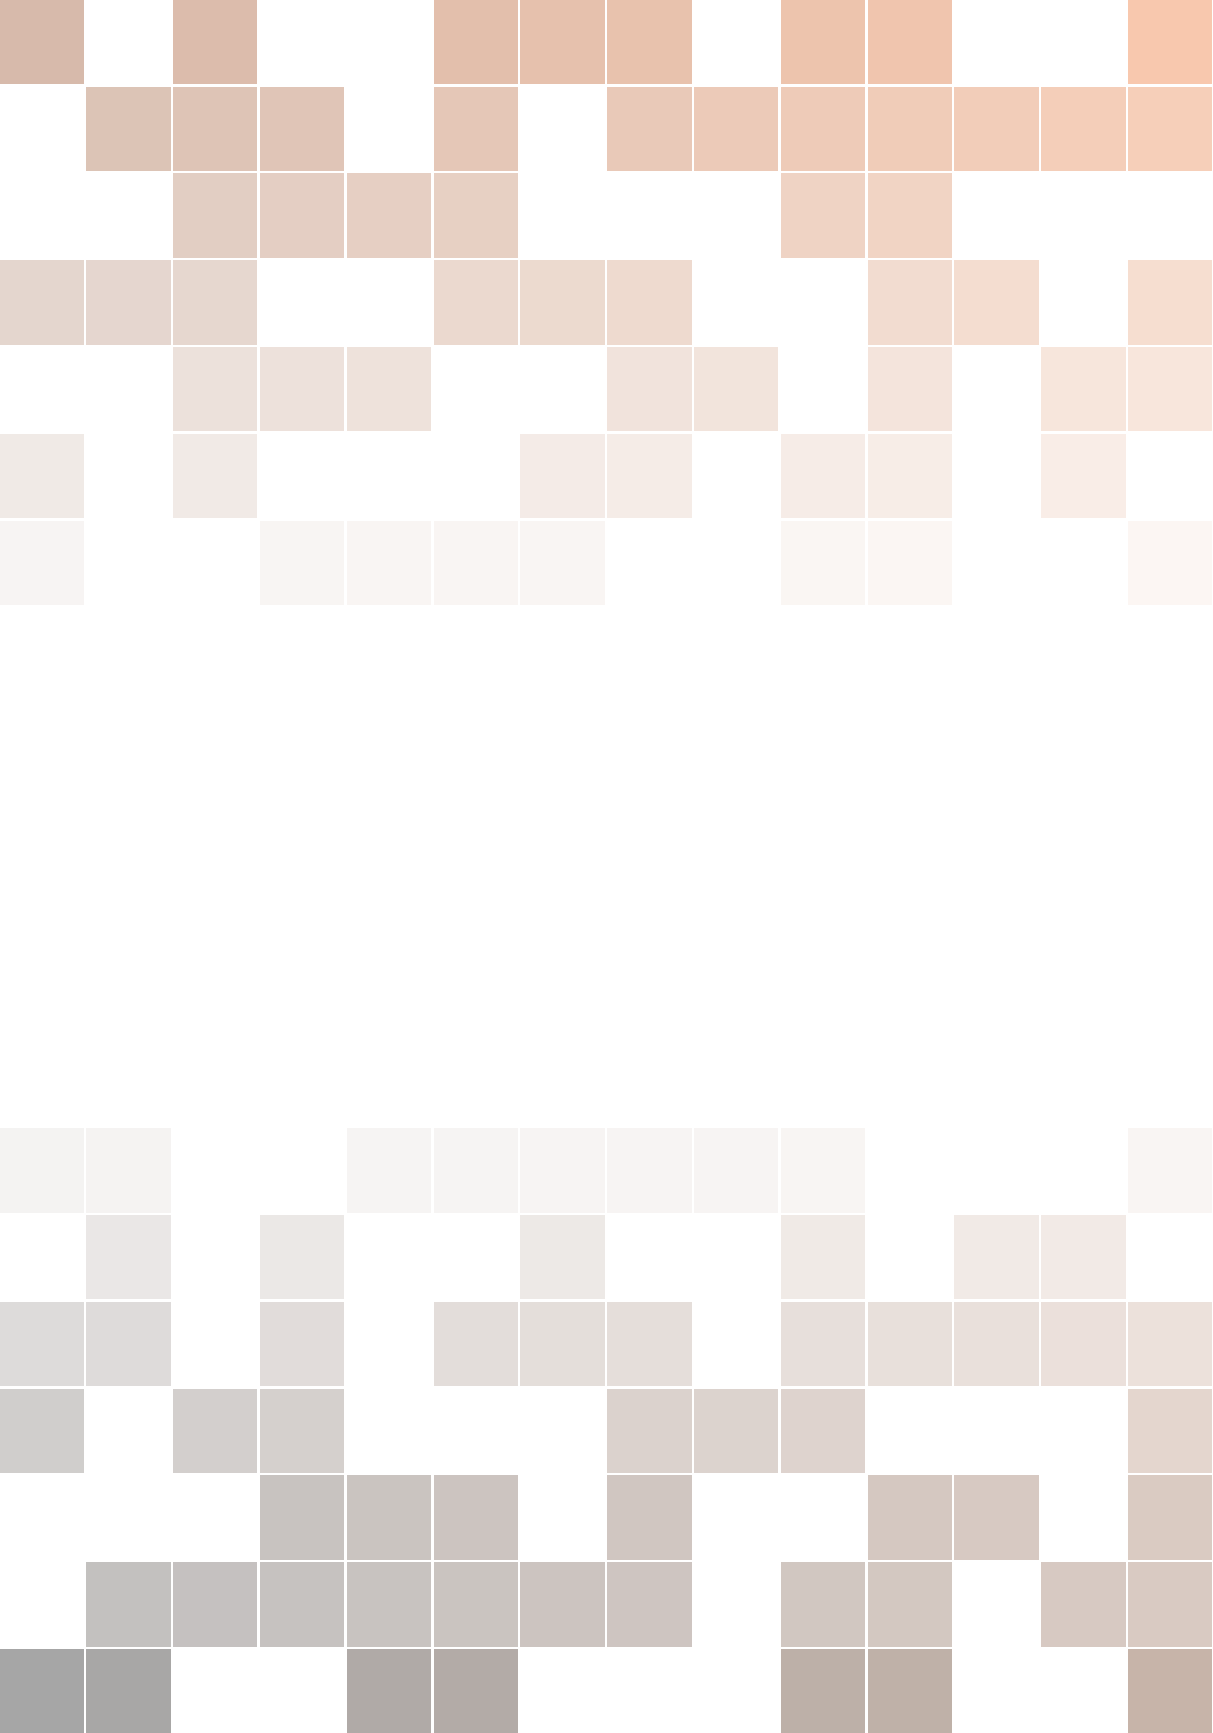
\includegraphics[width=\paperwidth]{images/background}}; % Background image
%\textsl{}
%      \draw[anchor=north] (midpoint) node [fill=ocre!30!white,fill opacity=0.6,text opacity=1,inner sep=1cm]{\Huge\centering\bfseries\sffamily\parbox[c][][t]{\paperwidth}{\centering Coding Interview Essentials\\[15pt] % Book title
%      {\Large - }\\[20pt] % Subtitle
%      {\huge Davide Spataro}}}; % Author name
%    \end{tikzpicture}};
%\end{tikzpicture}
%\vfill
%\endgroup


\includepdf[pages={2},fitpaper=true]{images/book_covers1.pdf}


\usechapterimagefalse % If you don't want to include a chapter image, use this to toggle images off - it can be enabled later with \usechapterimagetrue

%\chapterimage{images/header} % Table of contents heading image

\pagestyle{empty} % No headers

\tableofcontents % Print the table of contents itself

%\lstlistoflistings
%\listoffigures
%\listoftables

%\cleardoublepage % Forces the first chapter to start on an odd page so it's on the right

%pagestyle{fancy} % Print headers again
	%!TEX root = ../main.tex
%%%%%%%%%%%%%%%%%%%%%%%%%%%%%%%%%%
% Links:
%
% Difficulty: Companies: 
%%%%%%%%%%%%%%%%%%%%%%%%%%%%%%%%%%

\chapter{Number of Dice Rolls With Target Sum}
\label{ch:dice_rolls}
\section*{Introduction}

Dices have been around for quite a long time: the oldest dice known  were discovered in Iran, as part of a staggering five-thousand-year-old
 Backgammon\footnote{One of the oldest board game. A two-players game where pieces are moved around between twenty-four triangles according to the roll of two 6 faced-dice. The goal of each player is to remove all of their 15 pieces before the other player} set.

If we think about what a die is, the first thing that comes to mind is the fair $6$ faced-die (see Figure \ref{fig:dice_rolls:6faces_dice}), but potentially any polyhedron can be a die: consider for instance a  $20$-faced icosahedron (see Figure
\ref{fig:dice_rolls:20faces_dice}), or a $12$-faced dodecahedron (see Figure
\ref{fig:dice_rolls:12faces_dice}).
In this chapter's problem, we will use up to $30$ dice at the same time,
each with up to $30$ faces, and we are going to calculate the number of ways we can obtain a certain
target value when we throw them all at the same time.


\section{Problem statement}
\begin{exercise}
You have $d$ dice, and each die has $f$ faces numbered $1, 2, \ldots..., f$.
Write a function that returns the number of possible ways to roll the dice
so the sum of the upper
faces equals a given target number $t$. Because this number can be very large, the answer
should be returned modulo $10^9 + 7$.
	

	\begin{example}
		\hfill \\
		Given $d=1$, $f=6$ and $t=6$ the function should return $1$. Clearly, there is only one way to obtain $6$ when rolling a common $6$-face cubic die.
	\end{example}

	\begin{example}
		\label{ex:dice_rolls:example2}
		\hfill \\
		Given $d=2$, $f=6$ and $t=7$ the function should return $6$. Table \ref{tab:dice_rolls:arrangements_example2} lists all the possible ways of obtaining $7$ from two common $6$-face dice.
	\end{example}

	\begin{example}
		\hfill \\
		Given $d=2$, $f=3$ and $t=7$ the function should return $0$ because the highest number	obtainable by rolling two dices with three faces is $6$.
	\end{example}
\end{exercise}

\begin{table}
	\centering
	\begin{tabular}{|c|c|} 
	\hline
	\textbf{First die} & \textbf{Second die}  \\ 
	\hline
	1                  & 6                    \\
	2                  & 5                    \\
	3                  & 4                    \\
	4                  & 3                    \\
	5                  & 2                    \\
	6                  & 1                    \\
	\hline
	\end{tabular}
	\caption{Possible valide arrangements of two dice for the Example \ref{ex:dice_rolls:example2}}
	\label{tab:dice_rolls:arrangements_example2}
\end{table}


\section{Clarification Questions}

\begin{QandA}
	\item \begin{questionitem} \begin{question} What is the maximum number of dices, faces, and the highest target value possible?  \end{question} 	 
    \begin{answered}
		$30$,$30$ and $1000$, respectively.
	\end{answered} \end{questionitem}
	
\end{QandA}

\begin{figure}
	\centering
	\begin{subfigure}[t]{0.25\textwidth}
		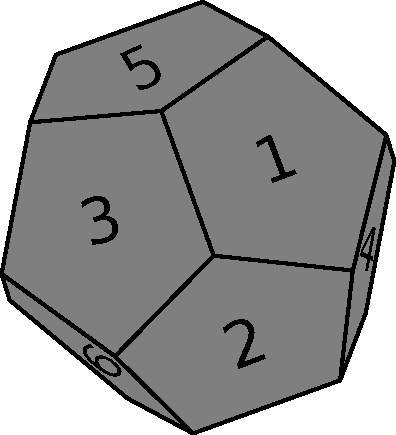
\includegraphics[width=1\linewidth]{sources/dice_rolls/images/3d_dices}
		\caption{Example of dice with $12$ faces.}
		\label{fig:dice_rolls:12faces_dice}
	 \end{subfigure}
	\hfill
	\begin{subfigure}[t]{0.25\textwidth}
		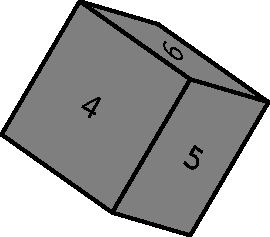
\includegraphics[width=1\linewidth]{sources/dice_rolls/images/cubic_dice}
		\caption{Example of common $6$ faces dice.}
		\label{fig:dice_rolls:6faces_dice}
	 \end{subfigure}
	 \hfill
	 \begin{subfigure}[t]{0.25\textwidth}
		 \includegraphics[width=1\linewidth]{sources/dice_rolls/images/icosahedron_dice}
		 \caption{Example of dice with $20$ faces.}
		 \label{fig:dice_rolls:20faces_dice}
	  \end{subfigure}
\end{figure}

\section{Discussion}
\label{dice_rolls:sec:discussion}

Let's start by noticing that the answer can be astronomically high, but more importantly, the number of possible value combinations resulting from rolling $d$ dices is even larger: if each die has
$f$ faces, then we are looking at $f^d$ possible distinct roll outcomes! 
During an interview, a brute-force approach, where we go over each and every possible roll outcome of the $d$ dice, is completely out of question  (considering the constraints on the maximum number of dices and faces we might get for input) unless we are willing to wait around  $6 \times 10^{18}$ years. Even if we implement this algorithm so that it can run on the fastest supercomputer available today (which is capable of a staggering $\approx450$ \footnote{\textbf{petaflop}: A petaflop is a measure of a computer's processing speed and can be expressed as: A quadrillion (thousand trillion) floating-point operations per second (FLOPS). A thousand teraflops. 10 to the 15th power FLOPS. 2 to the 50th power FLOPS. A huge number of operations per second.} operations per second), it would still require $\frac{30^{30}}{10e15}$s to run to completion. By that time, humanity will be long gone, the universe will be a dark and cold place, but most importantly, the position you are dreaming about will have gone to somebody else.

This type of \textit{"counting"} questions is usually (and crucially more efficiently) solved by using a dynamic programming
approach. In fact, this question shares a lot of similarities with the classical dynamic programming
\textit{Coin change} problem, to the point that we
could solve this one using the solution to the other. In fact we can stretch this reasoning so to consider the topic treated in this chapter to be a proper specialization of the *Coin
change* problem, where the number of available coins is equal to $d$
and the denomination of the coins are $1,2,\ldots,f$: we have coins of the same denomination as the
dice faces.




\subsection{Brute-force}
\label{dice_rolls:sec:bruteforce}


For science's sake, let's see how a brute-force approach would apply here. As we all know, a brute-force approach evaluates all possible outcomes of rolling $d$ dice and keeps
track of how many yield a total sum of $t$. When dealing with this kind of task, where you have to
enumerate/generate the elements of a given set, recursion is usually the way to go, especially if the elements (in this case a combination of face values) have a recursive definition.
In this specific case, we can generate all possible combinations of $d$ faces we can obtain from rolling $d$ dices by:

\begin{itemize}
	\item generate the combinations from rolling $d-1$ dice;
	\item create $f$ copies of them;
	\item prepend $1$ to the items of the first copy;
	\item prepend $2$ to the items of the second copy;
	\item $\ldots$  
	\item prepend $f$ to the items of the last copy.
\end{itemize}


For instance, we can generate all rolls outcome $3$ six-faced dice by:

\begin{enumerate}
	\item Generate all the outcomes for only $2$ of them $C_2$:\\
	$
	\!
	\begin{aligned}[t]
		C_2 =  \{
			& (1,1),(1,2),(1,3),	(1,4),	(2,1),	(2,2),	(2,3),	(2,4),\\
			&(3,1),	(3,2),	(3,3),	(3,4),	(4,1),	(4,2),	(4,3),	(4,4)\}
	\end{aligned}
	$ 
	

	\item Append $1$ to each of the elements of $C_2$:\\
	$
	\!
	\begin{aligned}[t]
		C_3^1 =  \{
			&(1,1,1),(1,1,2),(1,1,3),(1,1,4),(1,2,1),(1,2,2),(1,2,3),(1,2,4),\\
			&(1,3,1),(1,3,2),(1,3,3),(1,3,4),(1,4,1),(1,4,2),(1,4,3),(1,4,4)\}
	\end{aligned}
	$ 


	\item  Append $2$ to each of the elements of $C_2$: \\
	$
	\!
	\begin{aligned}[t]
		C_3^2 =  \{
			&(2,1,1),(2,1,2),(2,1,3),(2,1,4),(2,2,1),(2,2,2),(2,2,3),(2,2,4),\\
			&(2,3,1),(2,3,2),(2,3,3),(2,3,4),(2,4,1),(2,4,2),(2,4,3),(2,4,4)\}
	\end{aligned}
	$ 



	\item  Append $3$ to each of the elements of $C_2$:\\
	$
	\!
	\begin{aligned}[t]
		C_3^3 =  \{
			&(3,1,1),(3,1,2),(3,1,3),(3,1,4),(3,2,1),(3,2,2),(3,2,3),(3,2,4),\\
			&(3,3,1),(3,3,2),(3,3,3),(3,3,4),(3,4,1),(3,4,2),(3,4,3),(3,4,4)\}
	\end{aligned}
	$ 
	\item Prepend $4$ to each of the elements of $C_2$:\\
	$
	\!
	\begin{aligned}[t]
		C_3^4 =  \{
			& (4,1,1),(4,1,2),(4,1,3),(4,1,4),(4,2,1),(4,2,2),(4,2,3),(4,2,4),\\
			&(4,3,1),(4,3,2),(4,3,3),(4,3,4),(4,4,1),(4,4,2),(4,4,3),(4,4,4)\}
	\end{aligned}
	$ 

	\item  Finally, return $C_3 = \{C_2^1 \cup  C_2^2 \cup C_2^3 \cup C_2^4\}$
	
\end{enumerate}


The definition above is correct, but not very useful in practice: it requires making many copies
of a potentially very large (indeed exponential) set of items. We will therefore use a different approach that will still run in exponential time (this section is named brute-force after all), but it can be used as a basis for developing a more efficient DP solution.

We start by rolling the first die; clearly, we have $f$ possible values we can get, but
once the value for this specific die is set, say we got the value $x$, we are left with $d-1$ dices
to roll and we still have to make up for $t-x$ with the remaining $d-1$ dice in order to reach our target value
$t$. 
Once a die is rolled, we are left with exactly the original problem on a smaller number of dice
and target value. 
This is why recursion is handy as we can describe the solution to the entire problem in terms of solutions to
sub-problems.
We can continue this recursive process, rolling one die at a time, until we reach one of the following cases:
\begin{enumerate}
	\item $d<0$ or $t<0$ the answer is $0$. There is no solution to the problem when the number of
		dice to use is negative or the target number is negative.
	\item $t=0$. We have reached the target value $t$. If we have used \textbf{all} dice then we
		have a solution, otherwise we do not. In other words:
	\begin{itemize}
		\item  if $d=0$, we have used all $d$ dice and the sum is exactly equal to $t$. This is a
		valid combination. We have rolled $d$ dice and the sum of their faces is exactly equal to
		$t$.
		\item if $d>0$, we have not rolled all the dice, yet we have already reached our target
		value. If we continue to roll, we will generate a combination with a total sum higher than
		$t$. This is not a good combination.
	\end{itemize}
\end{enumerate}

The idea above can be better expressed using the recurrence relation shown in Equation
\ref{eq:dice_rolls:dpformula} where $S(d,t,f)$ is the number of ways one can obtain a target value
$t$ by throwing $d$ dice. Notice that the third parameter never changes, and thus it does not play a
dynamic role in the recurrence. 

\begin{equation}
	S(d,t,f)=\begin{cases}
		 1 \: \: \text{ if } \: d=t=0 \\
		 0 \: \: \text{ if } \: d=0, \: t>0 \\ \\
		\sum_{1}^{\min(f,t)} S(d-1,t-j,f)  \:\: \text{ otherwise}
	 \end{cases}
	\label{eq:dice_rolls:dpformula}
\end{equation}

Listing \ref{list:dice_rolls:bruteforce} shows a possible implementation of such idea. Please note
that this code is remarkably similar to the brute-force solution for the Coin Change problem in
Chapter \ref{ch:coin_change}. Section
\ref{sec:min_difficulty_job_scheduler:generate_all_combination} also discuss the problem of
generating combinations, and the material discussed there can be adapted and applied here.

\lstinputlisting[language=c++, caption={Brute-force (enumerating all possible combinations) solution for the problem of counting the number of dice rolls summing up to a target number $t$.},label=list:dice_rolls:bruteforce]{sources/dice_rolls/dice_rolls_solution1.cpp}


The time and space complexity of this approach are exponential and constant, respectively.
 
The proof of this  can be derived from the solution of the recurrence relation shown in Equation \ref{eq:dice_rolls:dpformula_complexity}:
\begin{equation}
	S(d,t) = S(d-1,t-1) + S(d-1,t-2)
\label{eq:dice_rolls:dpformula_complexity}
\end{equation}

where $S(d,t)$expresses the number of invocations of the function 
\inline{num_rolls_to_target_bruteforce}
for a given number of dice $d$ and target value $t$ when $f=2$. 
The resulting invocation tree is
complete and has height $h=t$ (assuming $d \leq t$, but the same reasoning can be applied in the
other cases). 
The cost of each node of the tree is $O(1)$. The number of nodes in such a tree is
exponentially proportional to its height. 



\subsection{Dynamic Programming - Recursive top-down}
\label{dice_rolls:sec:DP}
The brute-force solution we laid down in Section \ref{dice_rolls:sec:bruteforce} can  be turned into a nice and
efficient one with the help of DP, and in particular of memoization. As per many other problems
solvable with DP out there, the brute-force solution above can be turned into a much more
efficient one by simply realizing that the same sub-problems are solved over and over again.
For istance, imagine the case where $f=5$. We might end up solving the sub-problem where $d=1$ and
$t=3$  from the sub-problem where $d=2$, $t=4$ (by rolling the face with $1$), or from the
sub-problem $d=2$, $t=5$ (by rolling the face with $2$).

However, the maximum number of \textit{distinct} invocations for the function
\inline{num_rolls_to_target_bruteforce} is not larger than $30\times 1000 = 30000$: the maximum number of dice multiplied by the largest target value as these are the only function parameters varying during the execution. If we can somehow guarantee that no
duplicate work is done for a given $d$ and $t$, then we can get away with only $O(d\times t)$
function calls. 

Consider, for instance, what happens during the execution of the code
in Listing \ref{list:dice_rolls:bruteforce} for the following input:
\begin{itemize}
	\item $d = 3$
	\item $f = 6$
	\item $t = 12$
\end{itemize}


The function \inline{num_rolls_to_target_bruteforce(1,5,6)} is called  $6$ times and the
sub-problem \inline{num_rolls_to_target_bruteforce(1,4,6)} is solved $5$ times.
You can verify this yourself if you draw the recursion tree for \inline{num_rolls_to_target_bruteforce(3,6,12)}, or simply add a print statement at the beginning of the function.
All these duplicate calls are superfluous and they represent work that can be saved if the result of each sub-problem is stored into a
cache as shown in the following Listing.


The function subproblem \inline{num_rolls_to_target_bruteforce(1,5,6)} solved $6$ times and the
subproblem \inline{num_rolls_to_target_bruteforce(1,4,6)} is solved $5$ times. If you are not
convinced draw the recursion tree, or add a print statement at the beginning of the function. All
these superfluous execution can be avoided if the result of each of the subproblem is stored into a cache as shown in Listing \ref{list:dice_rolls:dp}. 

\lstinputlisting[language=c++, caption={Dynamic programming with memoization top-down recursive  solution for the problem of counting the number of dice rolls summing up to a target number $t$.},label=list:dice_rolls:dp]{sources/dice_rolls/dice_rolls_solution2.cpp}


This implementation is an almost identical copy
of the brute-force solution, except for the addition of a cache. Note how \textbf{before} actually trying
to compute the answer, we first look into the cache (see highlighted lines) to see if it is already present in the cache. If not, we solve the
problem and before returning the answer we \textbf{save} the result into the cache.

\section{Dynamic programming - Iterative bottom-up}
\label{dice_rolls:sec:bottom}

Turning the top-down-up solution shown in Section \ref{dice_rolls:sec:DP} into a bottom-up one is relatively easy: the recursive
definition of the solution (see Equation \ref{eq:dice_rolls:dpformula})   clearly shows that we can
calculate the answer for a given number of dice $d$ and a target value $t$ if we have already
calculated the values for targets $t-1, t-2, \ldots, t-f$ and $d-1$. We also know how to easily
calculate the answer for all possible target values when $d=0$ and $d=1$ and from there we can apply
the reasoning above. 
This is exactly the strategy that Listing \ref{list:dice_rolls:dpbottomup} implements.

\lstinputlisting[language=c++, caption={Dynamic programming bottom-up solution for the problem of counting the number of dice rolls summing up to a target number $t$.},label=list:dice_rolls:dpbottomup]{sources/dice_rolls/dice_rolls_solution3.cpp}

We use a 2D
table \inline{DP} (initialized with zeros) with $d+1$ rows and $t+1$ columns where each cell \inline{DP[i][j]}
corresponds to the solution of a sub-problem where $d=i$ and $t=j$. The first loop takes care of
filling the table with \textit{"known" values} for all sub-problems where $d=1$. If we only have a die with
$f$ faces, there is only one way we can achieve the target values $1,2,\ldots, f$ and no way to
obtain any higher values. The rest of the code fills the table one row at a time (one dice at a
time) by using the values of the previous row. 

The time and space complexity of this algorithm are $\Theta(dtf)$ and $\Theta(dt)$, respectively. 
However, the space complexity can be lowered easily
down  to $\Theta(t)$ because, as already mentioned, we only need space for two rows of the DP table:
one for the values of the current $d$ and one for the values at $d-1$.


%%%%%%%%%%%%%%%%%%%%%%%%%%%%%%%%%%%%%%%%%%%%
%               Appendices
%%%%%%%%%%%%%%%%%%%%%%%%%%%%%%%%%%%%%%%%%%%%

\chapter{Appendices}
%% @Author: Davide Spataro
% @Date:   2020-10-25 
% @Last Modified by:   Davide Spataro
% https://www.topcoder.com/community/competitive-programming/tutorials/dynamic-programming-from-novice-to-advanced/
% file:///home/knotman/Downloads/DYNAMIC_PROGRAMMING_-_ITS_PRINCIPLES_APPLICATIONS_.pdf
% http://smo.sogang.ac.kr/doc/bellman.pdf 
\section*{Dynamic Programming}
\label{sect:appendix:DP}

Dynamic programming (DP) is a popular technique for solving a certain class of
optimization problems efficiently and is accredited to the American Scientist
Richard Bellman\cite{bellman1954}. He conied the term DP in the context of
solving problems involving a serie of best decision one after the other. 
The word \textit{programming} can be a bit deceiving for
computer scientist of programmers in general but it has really little to do with
computer programming and it is infact intended as a set of rules to 
follow to solve a certain problem and it is refeered specifically to the
solution to find an optimal military schedule for logistics (and has more or
less the same meaning as linear programming or linear optimization).  These rules can of course be coded and
executed by a computer but can be easily followed on paper for instance. 
Dynamic programming is better thought as an optimization approach rather than an
method or framework where a complex optimization problem is transformed into a sequence of
smaller (and simpler) problems. The very essence of DP is its multi-stage
optimization procedure. DP does not provide directly with the
instruction on how to solve a particular problem, but instead provides a general
framework that requires creativity and non trivial effort/insights so that a
problem formulation can be adapted and casted within the DP framework bounds.
This is possibly the reason why DP is considered a rather hard topic and it is
particularly feared during interviews. 

This chapter is not intended to be a full treatement of DP, and we will
introduce and describe it to the level that is necessary to understand and
better tackle DP interview problems. For a more comprenshive material on DP
please refer to \cite{bellman1954, cormen2009}.

The gist of the DP approach is that we aim at breaking down a problem into
simpler sub-problems recursively. If it is possible to do so, then the problem
at hand is said to have the \textbf{optimal substructure} property i.e. it can
be solved by using optimal solution to subproblems. But having the optimal
substructure property alone is not enough to prefer a DP approach to another
when trying to solve the same problem. This is because DP really shines when a
problem also exposes the \textbf{overlapping subproblems} property i.e. when the
subproblems are reused several times. A classic example if the
Fibonacci Sequence. In order to calculate $F(n)$ we need to solve two subproblems:
$F(n-1)$ and $F(n-2)$ and adding them up. But for solving $F(n-1)$ we need to
solve $F(n-2)$ \textbf{again}. The value for the subproblem $F(n-2)$ is thus
reused and this makes the Fibonacci problem exposed the optimal substructure
property. 
Dynamic programming takes care of this fact by making sure of solving each
subproblem only once. Usually this can be achieved into two ways:
\begin{description}
    \item [Top-down] This is usually the easiest of the two, by being a direct
    derivation from the recursive formulation of the problem. If the problem can
    be formulated recursively in terms of solution then solution to subproblems
    can be \textit{memoized}\footnote{From the latin word \textit{memorandum}
    which means to be remembered. It is basically a way of remembering the
    result of a function for a certain set of inputs call by storing it in a
    cache.} in a cache. 
    When a subproblem is reused then the
    (potentially expensive) recursive call is avoided and the cached result is
    returned instead. 
    \item [Bottom-up] We can try to reformulate the problem by twisting and
    massaging  the  recursive formulation so that the subproblems are solved
    first (thus effectively removing the recursion) and build the solution to
    the bigger problem from the bottom. This is usually done by working in a
    sort of tabular form where entries of the table for larger problems are
    filled by using  entries for solution to smaller problems that we have
    already solved. For instance, when solving the problem of finding the
    $10^{th}$ Fibonacci number $F(10)$, we can start from the known values for
    $F(0)$ and $F(1)$ and working our way up to $F(2)$  by using $F(1)$ and
    $F(2)$. Once F(2) is ready we can move up to F(3), and so on when we have
    the values for $F(8)$ and $F(9)$ we proceed with calculating $F(10)$.
\end{description}

DP has found application in many field of science such as Control theory,
Bioinformatics AI and operations research. There are a number of problems in
computer science that can be solved by using DP such as the 
\begin{itemize}
    \item Longest Common (or increasing) Subsequence
    \item Weighted Interval Scheduling
    \item Chain Matrix Multiplication
    \item Subset sub
    \item String edit distance
    \item Coin change
    \item 0/1 knapsack problem
    \item Graph shortest path
\end{itemize}

In the next section we will shortly review a number of DP problem focusing on
the key ideas that allow a problem to be approached and solved  using DP.

\subsection*{Fibonacci Sequence}
Computing the $n^{th}$ number of the Fibonacci sequence is probably one of the
most common introductionary example of DP. The Fibonacci sequence recursive
formulation is ready to be solved using a top-down DP approach. Listing
\ref{list:app:dp:canonical} shows a C++ function that calculated the $n^{th}$ Fibonacci
number.
\lstinputlisting[language=c++, caption={Canonical recursive C++ implementation of a function returning the $n^{th}$ Fibonacci number.},label=list:app:dp:canonical]{/home/dspataro/git/algorithm_articles/sources/appendices/fibonacci_canonical.cpp}
Notice that for instance when $F(6)$ a call tree is produced where the same call
is repeated more than once as shown in the list below. $F(2)$ has been
calculated $5$ times!
\begin{itemize}
    \item $F(6) = F(5)+F(4)$
    \item $F(6) = (F(4)+F(3)) + (F(3)+F(2))$
    \item $F(6) = ((F(3)+F(2))+(F(2)+F(1))) + ((F(2)+F(1))+(F(1)+F(0)))$
    \item $F(6) = (((F(2)+F(1))+(F(1)+F(0)))+((F(1)+F(0))+F(1))) + (((F(1)+F(0))+F(1))+(F(1)+F(0)))$
    \item $F(6) = ((((F(1)+F(0))+F(1))+(F(1)+F(0)))+((F(1)+F(0))+F(1))) + (((F(1)+F(0))+F(1))+(F(1)+F(0)))$
\end{itemize}

Listing \ref{list:app:dp:fib} can be improved dramatically if we memoize the function calls
that have been already calculated. This way no duplicate work is done. W.r.t the
previous example, from the second time the value of $F(2)$ is needed, no
additional work is done, as the value in the cache is returned.
\lstinputlisting[language=c++, caption={Canonical recursive top-down Dynamic Programming C++ implementation of a function returning the $n^{th}$ Fibonacci number.},label=list:app:dp:fib]{/home/dspataro/git/algorithm_articles/sources/appendices/fibonacci_dp_top_down.cpp}

%\section{Prefix sum}
\label{sect:appendix:prefix_sum}
In computer science, the prefix sum, cumulative sum, inclusive scan, or simply scan of a sequence of numbers x0, x1, x2, ... is a second sequence of numbers y0, y1, y2, ..., the sums of prefixes (running totals) of the input sequence:
%% @Author: Davide Spataro
% @Date:   2020-03-30 17:18:14
% @Last Modified by:   Davide Spataro
% @Last Modified time: 2020-03-30 17:28:08
\section{Binary Search}
\label{sect:appendix:binary_search}
\lipsum{1}
%%%%%%%%%%%%%%%%%%%%%%%%%%%%%%%%%%%%%%%%%%%%
%               BIBLIOGRAPHY
%%%%%%%%%%%%%%%%%%%%%%%%%%%%%%%%%%%%%%%%%%%%

%
%from documentation
%\newacronym[⟨key-val list⟩]{⟨label ⟩}{⟨abbrv ⟩}{⟨long⟩}
%above is short version of this
% \newglossaryentry{⟨label ⟩}{type=\acronymtype,
% name={⟨abbrv ⟩},
% description={⟨long⟩},
% text={⟨abbrv ⟩},
% first={⟨long⟩ (⟨abbrv ⟩)},
% plural={⟨abbrv ⟩\glspluralsuffix},
% firstplural={⟨long⟩\glspluralsuffix\space (⟨abbrv ⟩\glspluralsuffix)},
% ⟨key-val list⟩}

\newacronym{cd}{CD}{compact disk}
\newacronym{utc}{UTC}{Coordinated Universal Time}
%\newacronym{adt}{ADT}{Atlantic Daylight Time}
%\newacronym{est}{EST}{Eastern Standard Time}
 
% Use the acronyms
\gls{utc} is 3 hours behind \gls{adt} and 10 hours ahead of \gls{est}.



%\addcontentsline{toc}{chapter}{\textcolor{ocre}{Glossary}}
%\printglossaries


%Print the glossary

\addcontentsline{toc}{chapter}{\textcolor{ocre}{Bibliography}}
%\chapter*{Bibliography}
%Print the glossary
\printbibliography	
	
%%%%%%%%%%%%%%%%%%%%%%%%%%%%%%%%%%%%%%%%%%%%
%               INDEX
%%%%%%%%%%%%%%%%%%%%%%%%%%%%%%%%%%%%%%%%%%%%	
	\cleardoublepage
	\phantomsection
	\setlength{\columnsep}{0.75cm}
	\addcontentsline{toc}{chapter}{\textcolor{ocre}{Index}}
	\printindex


	%\backmatter

\end{document}
